% Drawing 148/02-18 -- folder 148, batch 02, archive page 35 (PDF page 36).
% Transcription: sous les trois nombres, trois graphes : un sommet portant cinq arêtes libres ; deux sommets reliés, portant trois et deux arêtes libres ; trois sommets en chaîne, portant deux, une et deux arêtes libres, un petit trait oblique barrant l'arête libre du milieu.
% Kind: three graphs with free edges (types of five-pointed stable curves). Method 2 (schematic redraw from the facsimile). Status: ok.
% Notes: Ink. Graph 1: one vertex with five legs. Graph 2: two vertices joined by an edge, three legs on the left one and two on the right one. Graph 3: three vertices in a chain, two legs on the first, one on the middle, two on the last; a small oblique tick is scribbled across the middle leg and is drawn as a short stroke. The numbers 2, 1, 0 above the graphs are in the text and not drawn. The transcription says the central edge is barred; on the page the tick is on the middle leg, beside the middle vertex. The same three graphs stand in the margin of p. 30 (02-10). Redrawn 2026-11-12 (issue 128): to check again.
% Coordinates: 1 unit = 1 mm = 1/100 of the crop width, y downwards as on the crop (bbox in page fractions: [0.09, 0.465, 0.53, 0.555]).
% Redrawn by Claude (claude-fable-5-2), issue #128, 2026-11-12; not checked by a human; not compiled (no TeX in the session).
% Rights: reproduces part of the work -- behind RENDER_TRANSCRIPTS, never published by itself.
\documentclass[tikz,border=3pt]{standalone}
\usepackage{amsmath,amssymb}
\usetikzlibrary{patterns,arrows.meta}
\tikzset{pencil/.style={black!45}, struck/.style={black!35}, mpt/.style={circle,draw,inner sep=1.3pt}, pt/.style={circle,fill,inner sep=0.9pt}, opt/.style={circle,draw,fill=white,inner sep=1.1pt}, Rd/.style={red!75!black}, Gn/.style={green!45!black}, Br/.style={brown!70!black}}
\begin{document}
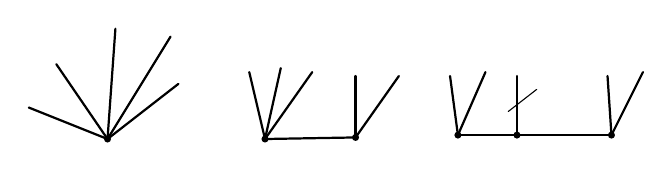
\begin{tikzpicture}[x=1mm,y=-1mm,line cap=round,line join=round,font=\small]
\coordinate (a) at (15.5,23.5);
\draw[thick] (a) -- (5.5,19.5);
\draw[thick] (a) -- (9,14);
\draw[thick] (a) -- (16.5,9.5);
\draw[thick] (a) -- (23.5,10.5);
\draw[thick] (a) -- (24.5,16.5);
\node[pt] at (a) {};
\coordinate (b) at (35.5,23.5);
\coordinate (c) at (47,23.3);
\draw[thick] (b) -- (c);
\draw[thick] (b) -- (33.5,15);
\draw[thick] (b) -- (37.5,14.5);
\draw[thick] (b) -- (41.5,15);
\draw[thick] (c) -- (47,15.5);
\draw[thick] (c) -- (52.5,15.5);
\node[pt] at (b) {};
\node[pt] at (c) {};
\coordinate (d) at (60,23);
\coordinate (e) at (67.5,23);
\coordinate (g) at (79.5,23);
\draw[thick] (d) -- (e) -- (g);
\draw[thick] (d) -- (59,15.5);
\draw[thick] (d) -- (63.5,15);
\draw[thick] (e) -- (67.5,15.5);
\draw (66.4,20) -- (70,17.2);
\draw[thick] (g) -- (79,15.5);
\draw[thick] (g) -- (83.5,15);
\node[pt] at (d) {};
\node[pt] at (e) {};
\node[pt] at (g) {};
\end{tikzpicture}
\end{document}
